\documentclass[11pt,letterpaper]{report}
%%%%%%%%%%%%%%%%%%%%%%%
%% Page layout
\usepackage{graphics,graphicx,wrapfig}
\usepackage[letterpaper, margin=2.5 cm, headheight=4 cm, top= 6cm]{geometry}
\setlength{\parindent}{0pt}
\usepackage{parskip}
\setlength{\parskip}{0.5em}

\usepackage{fancyhdr}

\fancyhf{}
\fancyhead[L]{

\includegraphics[height=3 cm]{../Figures/Brown_Letterhead/H_2c_Pos}
\\
}
%
\fancyhead[C]{
\parbox[b][3.5cm][t]{4cm}{
\begin{flushright}
Haneesh Kesari
\\
Assistant Professor 
\\
of Engineering
\\
\end{flushright}
}
}
%
\fancyhead[R]{
\parbox[b][3.5cm][t]{6cm}{
\begin{flushleft}
School of Engineering
\\
Brown University
\\
184 Hope Street, B\&H 612
\\
Providence, RI 02912
\\
Phone: 401-863-1418
\\
Email: Haneesh\_Kesari@brown.edu
\\
\end{flushleft}
}
}

\fancypagestyle{plain}{
\fancyhf{} % remove everything
%
\renewcommand{\headrulewidth}{0pt} % remove lines as well
%
\renewcommand{\footrulewidth}{0pt}
%
\fancyfoot[R]{\thepage / \pageref{LastPage}}
}

%% Fonts
\usepackage{amssymb,amsfonts,amsmath,amsthm}
\usepackage[T1]{fontenc}
\usepackage{mathptmx}
\usepackage{cmbright}
\usepackage{bm}

\usepackage{sectsty}
\sectionfont{\fontsize{16}{16}\selectfont}

%% typesetting
\usepackage{tabto}

%% colors
\usepackage{xcolor}
\definecolor{DarkRed}{rgb}{0.62, 0.16, 0.09}

%% referencing
\usepackage{nameref}
\usepackage{lastpage}
\usepackage[superscript,biblabel]{cite}
\usepackage[colorlinks=true,urlcolor=DarkRed,linkcolor=DarkRed,citecolor=black]{hyperref}

%% enumerate
\usepackage{enumerate}
\usepackage{enumitem}

%% floats
\usepackage{float}
\usepackage[font=footnotesize, labelfont={bf},labelsep=period]{caption}
\usepackage{booktabs}
\usepackage{threeparttable}

%% custom commands
\newcommand{\loc}{\textit{LoC}}

\newcommand{\norm}[1]{\ensuremath \lVert #1 \rVert}

\newcommand{\ex}{{\bm{\hat{e}}}_1}
\newcommand{\ey}{{\bm{\hat{e}}}_2}
\newcommand{\ez}{{\bm{\hat{e}}}_3}
\newcommand{\ei}{{\bm{\hat{e}}}_i}
\newcommand{\ej}{{\bm{\hat{e}}}_j}
\newcommand{\er}{{\bm{\hat{e}}}_r}
\newcommand{\et}{{\bm{\hat{e}}}_\theta}
\newcommand{\ep}{{\bm{\hat{e}}}_\phi}

\usepackage{xspace}
\newcommand{\TA}{\textit{Ta.\@}\xspace}
\newcommand{\EA}{\textit{Ea.\@}\xspace}


\begin{document}
%%%%%%%%%%%%%%%%%%%%%%%%%%%%%%%%%%%%%%%%%%%%%%%%%%%%%%
%%%%%%%%%%%%%%%%%%%%%%%%%%%%%%%%%%%%%%%%%%%%%%%%%%%%%%
%%%%%%%%%%%%%%%%%%%%%%%%%%%%%%%%%%%%%%%%%%%%%%%%%%%%%%
\thispagestyle{fancy}
\phantom{x}
\vspace{4em}
Author response letter to Reviewers

Regarding: Revision of original research article \textit{``Architecture in Stiff Biological Materials: a Template for Toughness Enhancement, or a Siren Song?''}

\vspace{4em}
Dear Reviewers,

We thank you for your very valuable feedback. In response to your feedback, we have made the revisions listed in the section \textit{List Of Changes} (\loc) on page \pageref{LoCpage} of this letter. The regions containing our revisions are marked in red in the revised manuscript. Our responses to Reviewer \#1, \#2 and \#3's comments can be found starting on pages \pageref{rev1}, \pageref{rev2} and \pageref{rev3}, respectively. Through these changes and our responses to your comments, we hope that we have addressed all of your concerns.

We thank you for your consideration of our revised manuscript.

\vspace{2em}
Sincerely,

Haneesh Kesari, Michael A. Monn, Kaushik Vijaykumar, and Sayaka Kochiyama


%%%%%%%%%%%%%%%%%%%%%%%%%%%%%%%%%%%%%%%%%%%%%%%%%%%%%%
%%%%%%%%%%%%%%%%%%%%%%%%%%%%%%%%%%%%%%%%%%%%%%%%%%%%%%
%%%%%%%%%%%%%%%%%%%%%%%%%%%%%%%%%%%%%%%%%%%%%%%%%%%%%%
\clearpage
\pagestyle{plain}
\newgeometry{margin=2.5 cm}
%%%%%%%%%%%%%%%%%%%%%%%%%%%%%%%%%%%%%%%%%%%%%%%%%%%%%%
\section*{List of Changes}
\label{LoCpage}

{\bf Changes in response to major Reviewer criticisms}
\begin{enumerate}[label=\textit{Mc.\arabic*}]
%
\item \label{Mc01} In response to Reviewer \#1's comment (listed as comment~\ref{r1c1} of this letter) regarding our finding that the toughness enhancement provided by the \EA spicule's architecture is small compared to the enhancements observed in other biological materials, we have added two sentences to the abstract that clarifies the scope of these findings.
%
\item \label{Mc02} In response to Reviewer \#1's comment (listed as comment~\ref{r1c1} of this letter) regarding our finding that the toughness enhancement provided by the \EA spicule's architecture is small compared to the enhancements observed in other biological materials, we have added several sentences to the second to last paragraph of the introduction to point out that we observe a substantial increase in fracture initiation toughness for short notches and to compare this increase to previous predictions in literature.
%
\item \label{Mc03} In response to Reviewer \#1's comment (listed as comments~\ref{r1c2}--\ref{r1c5} of this letter) regarding the length of notches used in this work, we performed additional experiments on 10 \EA and 14 \TA spicules and modified the fifth paragraph of Section 2.3 to discuss the increase in fracture initiation toughness observed at small $\alpha$.
%
\item \label{Mc04} In response to Reviewer \#1's comment (listed as comments~\ref{r1c2}--\ref{r1c5} of this letter) regarding the length of notches used in this work, we added a paragraph following the fifth paragraph of Section 2.3 to discuss possible reasons for the increase in $R(0)$ at small $\alpha$ and connect this observed increase to previous works.
%
\item \label{Mc1} In response to Reviewer \#2's suggestion (listed as comment~\ref{r2c2} of this letter) regarding identifying the limitations of the Regularized Variational Fracture Theory, we have added a paragraph to Supplementary Information Section S4.1 that discusses the primary limitation of RVFT as it applies to the current study. 
%
\item \label{Mc2} In response to Reviewer \#2's comment (listed as comment~\ref{r2c7} of this letter) regarding inclusion of statistics both for measurements obtained in this work and those referenced from other works, we have included a new table (Table 1 in the revised version) that summarizes statistical data for specimen geometry (i.e., span, diameter, and notch length) as well as references to this table in the text.
%
\item \label{Mc3} In response to Reviewer \#2's comment (listed as comment~\ref{r2c7} of this letter) regarding inclusion of statistics both for measurements obtained in this work and those referenced from other works, we have included the standard error of the notch root radius measurements in paragraph 4 of Section 2.3 in the revised version.
%
\item \label{Mc4} In response to Reviewer \#2's comment (listed as comment~\ref{r2c7} of this letter) regarding inclusion of statistics both for measurements obtained in this work and those referenced from other works, we have modified Table 2 in the revised version to include statistical data when available for the values of $R(0)$ and $\left< R\right>$ for the other SBMs shown in Figure 8.
%
\end{enumerate}

\clearpage
{\bf Changes in response to minor Reviewer criticisms}
\begin{enumerate}[label=\textit{mc.\arabic*}]
%
\item \label{mc00} Added Sayaka Kochiayama as a co-author on the paper following her contributions preparing, testing, and analyzing the 10 additional \EA and 14 additional \TA specimens in response to Reviewer \#1's criticism that is listed as comments \ref{r1c2}--\ref{r1c5} of this letter.
%
\item \label{mc01} Modified Table 1 to reflect the 10 additional \EA specimens and 14 additional \TA specimens that we tested.
%
\item \label{mc02} Updated number of \EA and \TA spicule specimens in the first paragraph of the Results section to reflect the additional \EA and \TA specimens that we tested.
%
\item \label{mc03} Updated the measurements of $r_n$ in the fourth paragraph of Section 2.3 to reflect the additional \EA and \TA specimens that we tested.
%
\item \label{mc04} Changed the number of specimens excluded from the calculation of $R(0)$ due to excessive notch root radius or lack of pop-in in paragraph four of Section 2.3.
%
\item \label{mc05} Updated the values of $R(0)$ in paragraph five of Section 2.3 to reflect the additional \EA and \TA specimens that we tested.
%
\item \label{mc06} Updated the number of specimens used to compute $\left< R \right>$ and values of $\left< R \right>$ in Section 2.4 to reflect the additional \EA and \TA specimens that we tested.
%
\item \label{mc07} Modified the values for the fracture toughness enhancements given in Section 2.5 and added a sentence to describe the additional enhancement in $R(0)$ observed for short notches to address Reviewer \#1's criticism that is listed as comments~\ref{r1c2}--\ref{r1c5} of this letter.
%
\item \label{mc08} Added an additional point to Figure 8 to identify the approximate value of the maximum $R(0)$ enhancement observed in the \EA spicules.
%
\item \label{mc09} Updated notch width values in Section 5.2 to reflect the additional \EA and \TA specimens that we tested.
%
\item \label{mc010} Updated Figure 7 to include the additional \EA and \TA specimens that we tested.
%
\item \label{mc011} Updated Tables S1 and S2 in the Supplementary Information to include information for the additional \EA and \TA specimens that we tested.
%
\item  \label{mc1} Added a sentence to the first paragraph of the introduction to address Reviewer \#2's criticism that is listed as comment~\ref{r2c3} of this letter.
%
\item  \label{mc2} Modified Figure 3 and its caption, and added a figure reference to the fourth paragraph of the introduction to address Reviewer \#2's criticism that is listed as comment~\ref{r2c4} of this letter.
%
\item  \label{mc3} Modified the caption of Figure 8 and added a figure reference to the second paragraph of Section 2.5 to address Reviewer \#2's criticism that is listed as comment~\ref{r2c5} of this letter.
%
\item  \label{mc4} Modified Figure 9 to address Reviewer \#2's criticism that is listed as comment~\ref{r2c6} of this letter.
%
\item  \label{mc5} Modified the caption of Figure S1 to address Reviewer \#2's criticism that is listed as comment~\ref{r2c8} of this letter.
%
\item  \label{mc6} Modified the sentence on line 76 of the original version to address Reviewer \#2's criticism that is listed as comment~\ref{r2c9} of this letter.
%
\item  \label{mc7} Corrected typos to address Reviewer \#2's criticism that is listed as comment~\ref{r2c10} of this letter.
%
\item  \label{mc8} Added information on standard deviation and sample numbers to Table 2 in the revised version.
%
\end{enumerate}

\clearpage
%%%%%%%%%%%%%%%%%%%%%%%%%%%%%%%%%%%%%%%%%%%%%%%%%%%%%%
\section*{Response to Reviewer \#1's comments}
\label{rev1}

\begin{enumerate}[label=\textit{1.\arabic*},wide, labelwidth=!, labelindent=0pt]
\item \label{r1c1} {\bf ``From their measurements, they conclude that the layered structure does not improve the fracture toughness.''}

The primary finding of our work is that, in contrast to previous speculations, the cylindrically layered architecture of the \textit{Euplectella aspergillum} spicules does not provide the same magnitude of toughness enhancements that are observed in other biological materials with layered architectures. We do, in fact, measure a significant increase in both fracture initiation toughness and average crack growth resistance. However, these enhancements are much smaller (by up to 2 orders of magnitude) compared to materials like nacre, bone, and conch shell to which the spicules have been previous compared \cite{mayer2011new, mayer2005rigid}.

We do not wish to mislead the reader in this regard and have consequently made two changes, which are listed as \ref{Mc01} and \ref{Mc02} in the \textit{LoC} to clarify this finding.
%
Through change \ref{Mc01} we have added a paragraph in the introduction to clarify that we did measure up to a ten fold increase in fracture initiation toughness but that this increase is small compared to the increases observed in nacre and bone.
%
Through change \ref{Mc02} we have added a paragraph to Section 2.5 that compares the increase in fracture initiation toughness that we observed to increases observed in conch, antler, and nacre.

\item \label{r1c2} {\bf ``A layered structure improves fracture toughness and damage tolerance only, if an existing crack has to cross the layers, i.e. when it propagates perpendicular to the spatial variation of the material properties, see e.g. Fratzl et al. Advanced Materials 2007 and ref. [8].''}

We agree with the Reviewer that many toughening mechanisms (e.g., the Cook-Gordon mechanism \cite{cook1964mechanism} and crack tip shielding \cite{fratzl2007hindered}) require that a crack to propagate perpendicular to the spatial variation in material properties. In this work we presented measurements of both fracture initiation toughness (Section 2.3) and average crack growth resistance (Section 2.4). Whether a crack propagates \emph{roughly} perpendicular to the \EA spicule's cylindrically layered architecture depends on the location of the crack within the spicule and the direction of its growth. For this reason, we will address fracture initiation toughness and average crack growth resistance separately in the following paragraphs.

In the case of average work of fracture, regardless of whether the a notch extends into the \EA spicule's core it must propagate perpendicular to the layers once it reaches the other side of the core in order to completely cleave the spicule's cross-section. Therefore, the effects of the aforementioned toughening mechanisms would contribute to the average work of fracture regardless of the initial notch length. 

In the case of fracture initiation toughness, to satisfy the requirement that the crack \emph{initially} propagate perpendicular to the layered architecture, the initial notch should not extend into the spicule's monolithic core. In a previous work \cite{monn2015new}, it has been shown that the ratio of the core's diameter to the spicule's diameter is relatively constant with a mean value of 0.41 and a standard deviation of 0.07 ($N$=116). From this measurement, we found that notches whose lengths exceed 0.3 times the spicule's diameter will extend into the core. In the original version of the paper there were seven \EA spicules with values of $\alpha\leq$0.3, five of which produced valid measurements of fracture initiation toughness. The fracture initiation toughness of these five spicules was similar to that of the other spicules with larger values of $\alpha$. However, in response to this comment we have conducted additional experiments with values of $\alpha<$0.3 in order to better assess the effect of the architecture on fracture initiation toughness. Specifically, we have conducted tests on ten additional \EA specimens and fourteen additional \TA specimens (see Tables S1 and S2 in the revised manuscript, and Figure 7). We found that for values of $\alpha\leq$0.1 the \EA spicules displayed a substantial increase in fracture initiation toughness with the largest value being approximately ten times greater than the corresponding value for the \TA spicules. We do not believe that this new data invalidates our previous findings since the increase in fracture initiation toughness for short notches (up to 10 fold increase) was still relatively small compared to the toughness enhancements observed in bone (up to 20 fold increase \cite{nalla2005mechanistic}) and nacre (up to 250 fold increase \cite{jackson1988mechanical})

We thank the Reviewer for this feedback, without which we would not have observed this increase in fracture initiation toughness for very short notches. In response to this comment we have made four changes, which are listed as \ref{Mc01}--\ref{Mc04} in the \textit{LoC}.

Through changes \ref{Mc01} and \ref{Mc02} we have pointed out both in the introduction and the abstract that for very short notches, the \EA spicule's architecture does appear to increase their fracture initiation toughness by up to a factor of 10.

Through changes \ref{Mc03} and \ref{Mc04} we have described these new results in detail. Specifically, we point out that for $\alpha>$0.1 the fracture initiation toughness of the \EA spicules is not significantly different than that of the \TA spicules. However, for specimens in which $\alpha<$0.1 the \EA spicules display a substantial increase in fracture initiation toughness. We then remark that this observed increase is consistent with a previously proposed model for fracture initiation toughness enhancement \cite{fratzl2007hindered, kolednik2014improvements, kolednik2011bioinspired}.

\item \label{r1c3} {\bf ``Hereby, the notch length a varies between 0.27 and 0.4 times the diameter of the spicule (Fig. 7). This means that the cut reaches the silica core of the spicule where no protein interlayers are present and the interlayers near the outside do not lie perpendicular to the crack growth direction, compare Fig. 1 to Figs. 3 and 6.''}

In the data presented in the original version of the manuscript, the notch length varied between 0.18 and 0.64 (see Table S1). This data is also represented in Figure 7, as stated by the Reviewer. In a previous work \cite{monn2015new}, it has been shown that the ratio of the core's diameter to the spicule's diameter is relatively constant with a mean value of 0.41 and a standard deviation of 0.07 ($N$=116). From this measurement, we found that notches whose lengths exceed 0.3 times the spicule's diameter will extend into the core. The original version of this manuscript contained fracture initiation toughness measurements from five \EA spicules for which $\alpha<$0.3. The fracture toughness of these five \EA spicules was not significantly higher than the other spicules that we tested.

However, in response to this feedback, we have performed fracture tests on 10 additional \EA spicules and 14 additional \TA spicules for which $\alpha$ ranged from 0.07 to 0.19. These additional experiments revealed, as the Reviewer suggested, that for very short notches ($\alpha<$0.1) the \EA spicules architecture has a substantial effect on its fracture initiation toughness. We observed up to a ten-fold increase in fracture initiation toughness in these additional tests. 

In response to this feedback, we have incorporated the additional data into the revised version of the manuscript and have made four major changes, enumerated as \ref{Mc01}--\ref{Mc04} in the \textit{LoC}, and 11 minor changes, enumerated as \ref{mc01}--\ref{mc011} in the \textit{Loc}. Through these changes we describe the observed increase in fracture initiation toughness for small $\alpha$ and its potential causes. While this new finding contrasts with the data presented in the original version it does not invalidate our original assertion that the \EA spicule's architecture does not provide the same magnitude of enhancements observed in many other biological materials. For example, while the \EA spicule's architecture can provide a ten fold enhancement to fracture initiation toughness, this still pales in comparison to the 250 fold enhancement observed in nacre \cite{jackson1988mechanical}. Through these changes we also reaffirm this assertion in light of these new observations.

\item \label{r1c5} {\bf ``Therefore, it is clear that the fracture resistance comes close to the fracture toughness of homogeneous calcite.''}

In this manuscript we do not compare the fracture toughness of the \EA spicules to that of calcite. Since the \EA and \TA spicules are composed primarily of silica (i.e., partially hydrated SiO$_2$), we provide reference values for the fracture toughness (both initiation toughness and average crack growth resistance) of synthetic glass. However, the spicule's chemical composition is distinct from synthetic glass. Unlike synthetic glass, the Ea. spicules are composed of hydrated silica that is precipitated onto a proteinaceous scaffold \cite{ehrlich2010chitin}. The effect of this scaffold on the mechanical properties of the spicule's silica is not fully understood. For this reason we chose to compare the \EA spicules to \TA spicules, which have been shown to have a similar chemical composition. We discuss this choice in detail in Section 2.5 of both the original and revised manuscript.

\item \label{r1c6} {\bf ``The increase of fracture toughness due to soft and/or compliant interlayers has been demonstrated experimentally in several papers, e.g. in Sistaninia et al., Composite Structures 2018.''}

We thank the Reviewer for pointing us to the work of Sistaninia et al and suggesting a link between our findings and theirs. We have discussed this link and related works in Section 2.3 of the revised manuscript. Specifically, we state that it has been shown that when a crack grows through a solid consisting of planar layers of a stiff material, separated by thin, compliant or weak interlayers, the solid exhibits a larger fracture initiation toughness than the bulk material \cite{fratzl2007hindered, kolednik2014improvements, kolednik2011bioinspired}. This apparent toughness enhancement is a result of the energy release rate decreasing when the crack impinges on a compliant interlayer. Furthermore, this mechanism has been observed experimentally in bioinspired composites \cite{zechner2013fracture, sistaninia2018design}.

\item \label{r1c7} {\bf ``p.4, l.54: `Roughly speaking, fracture toughness---also known as crack growth resistance, R---is the amount of energy that a crack consumes to grow its area by a unit amount.' This is valid for brittle, homogeneous materials only, but not for inhomogeneous materials where a crack has to cross soft interlayers.''}

In this work we consider the often ambiguously-defined term ``fracture toughness'' to be synonymous with the crack growth resistance, $R$. By Irwin's adaptation of Griffith's theory of fracture, $R$ is defined as the energy that a crack consumes to grow by a unit amount \cite{anderson2017fracture, lawn1993fracture}. Originally, $R$ was taken to be constant and equal to the surface energy of the material \cite{griffith1921phenomena}. This description is valid for perfectly brittle materials. However, Irwin and Orowan extended this concept to include other dissipative processes acting near a crack tip \cite{anderson2017fracture}. This allows the concept of the crack growth resistance to be extended beyond materials that are homogeneous and perfectly brittle.

Under this description, a material's ``fracture toughness'' can vary as a crack propagates and the term $R$ encapsulates the combined effects of surface energy, intrinsic toughening mechanisms like crack tip shielding due to elastic inhomogeneity, and extrinsic mechanisms like crack bridging \cite{evans1990perspective, lawn1993fracture}. Thus, $R$ is meant to encapsulate a variety of energy sinks that augment the material's inherent surface energy \cite{lawn1993fracture}. These energy sinks are often associated with the material's microstructure or architecture. For example, in Section 3 we discuss the crack arrest and re-nucleation mechanism that increases $R$ as a crack impinges on a weak interlayer within a material. In the revised version we have also added a discussion of the effect of crack tip shielding due to the presence of compliant or weak interlayers (see change \ref{Mc04} in the \textit{LoC}).

\item \label{r1c8} {\bf ``p.9 Fig 5 and p.11: It is wrong to compute the fracture initiation toughness of the E. aspergillum spicule from Eq. (2). The change in potential energy and the crack extension during the the pop-in only gives the crack growth resistance for the first crack growth increment after fracture initiation.''}

We agree with the Reviewer that the change in potential energy and crack extension during pop-in only provide the value of $R$ for the first crack growth increment after initiation. By definition, the value $R(\Delta a)$ as the crack length $\Delta a$ tends to zero (i.e., the first increment following initiation) is the material's fracture initiation toughness. Therefore, based on their second statement, we do not understand why the Reviewer believes that Eqn. (2) cannot be used to compute the fracture initiation toughness.

To clarify, we derive Eqn. (2) directly from Griffith's criterion that the necessary condition for crack growth is satisfied when the energy release rate is equal to the material's crack growth resistance. If both the energy release rate and the crack growth resistance vary with crack extension $\Delta a$, then Griffith's criterion can be expressed as
%
\[-\frac{d \Pi (\Delta a;\; w_s)}{d\Delta A(\Delta a;\; a,\;D)}=R(\Delta a),\]
%
where $\Pi(\Delta a;\;w_s)$ is the system's potential energy when the crack's length is $\Delta a$ and the applied displacement is $w_s$, and $\Delta A(\Delta a;\; a,\;D)$ is the change in fracture surface area associated with a change in crack length of $\Delta a$. By setting $\Delta a$=0 and writing the derivative with respect to $\Delta a$ instead of $\Delta A$, we immediately recover Eqn. (2). Therefore, the fracture initiation toughness for a specimen with a circular cross-section containing an edge crack is given by Eqn. (2).


\end{enumerate}

\clearpage
%%%%%%%%%%%%%%%%%%%%%%%%%%%%%%%%%%%%%%%%%%%%%%%%%%%%%%
\section*{Response to Reviewer \#2's comments}
\label{rev2}

\begin{enumerate}[label=\textit{2.\arabic*},wide, labelwidth=!, labelindent=0pt]
\item \label{r2c1} {\bf ``On the use of the variational fracture method (VFM) to discuss and explain the results. The set of past works from Ambrosio and Tortorelli, and later Francfort and Marigo (1998 \& 2000) report numerical evidence for the variational fracture theory validation. While I certainly acknowledge the power and refinement of this method, I wonder whether after 18-20 years, the authors could have considered adding experimental validation. This would be certainly pertinent here considering the VFM is now applied to a biological layered material. Would for example, the fabrication and test of a simple synthetic analog, i.e. an artificial layered beam with controlled elastic properties for its bulk solid and its thin interlayer, be brought further evidence for the VFM accuracy and use in this work?''}

We agree with the Reviewer that experimental validation is extremely important for verifying the predictive capabilities of any computational tool. While we did not include this information in the manuscript, we have carried out simulations to validate our finite element implementation of Regularized Variational Fracture Theory (RVFT) against experimentally observed crack paths in brittle materials. In Figure~\ref{Fig4} (a) of this letter, we show the crack path predicted by the RVFT for a solid subjected to mode-II loading. The red region indicates the cracked region, where the damage variable $d=1$. We measured the crack initiation angle from the simulations to be $69.2^\circ$. This angle compares well with previous experimental measurements of $67^\circ$--$72.5^\circ$ as well as the angle of $70.5^\circ$ predicted by the maximum tangential stress criterion \cite{erdogan1963crack}. These results show that the RVFT can predict the crack initiation angle without any additional/\emph{ad hoc} initiation criterion. 

In order to determine the accuracy of crack path prediction after initiation, we used our RVFT to simulate crack growth in a solid with heterogeneities---in this case, holes. Specifically, we compared results from our RVFT to those obtained from three point bending tests performed on Poly(methyl methacrylate) (PMMA) bars with three holes drilled in them \cite{bittencourt1996quasi}. An illustration of the specimen geometry is shown in Figure~\ref{Fig4} (b.i) of this letter. The crack path measured from the experiment is adapted from \cite{bittencourt1996quasi} in Figure~\ref{Fig4} (b.ii) of this letter, where the region shown corresponds to the blue region indicated in subfigure (b.i). The crack path from our RVFT simulation is shown in Figure~\ref{Fig4} (b.iii) of this letter. In Figure~\ref{Fig4} (b.iv) of this letter, we compared the angle $\theta$ between the tangent to the crack path and the $x$-axis predicted by RVFT (grey curve) to the experimental measurements (red dots).

Additionally, RVFT-based simulations have been quantitatively validated against experiments in brittle materials by other researchers as well \cite{mesgarnejad2015validation}. One example from \cite{mesgarnejad2015validation} is shown in Figure~\ref{Fig4} (c) of this letter. The geometry and loading conditions are shown in subfigure (c.i). A comparison of the crack path predicted by the RVFT (denoted by a red curve) and the experiments (denoted by dashed black curves) is shown in Figure~\ref{Fig4} (c.ii) of this letter. Based on these results, we conclude that RVFT can accurately predict crack propagation in brittle materials, even in the presence of heterogeneities like holes.

\begin{figure}[hb!]
	\centering
	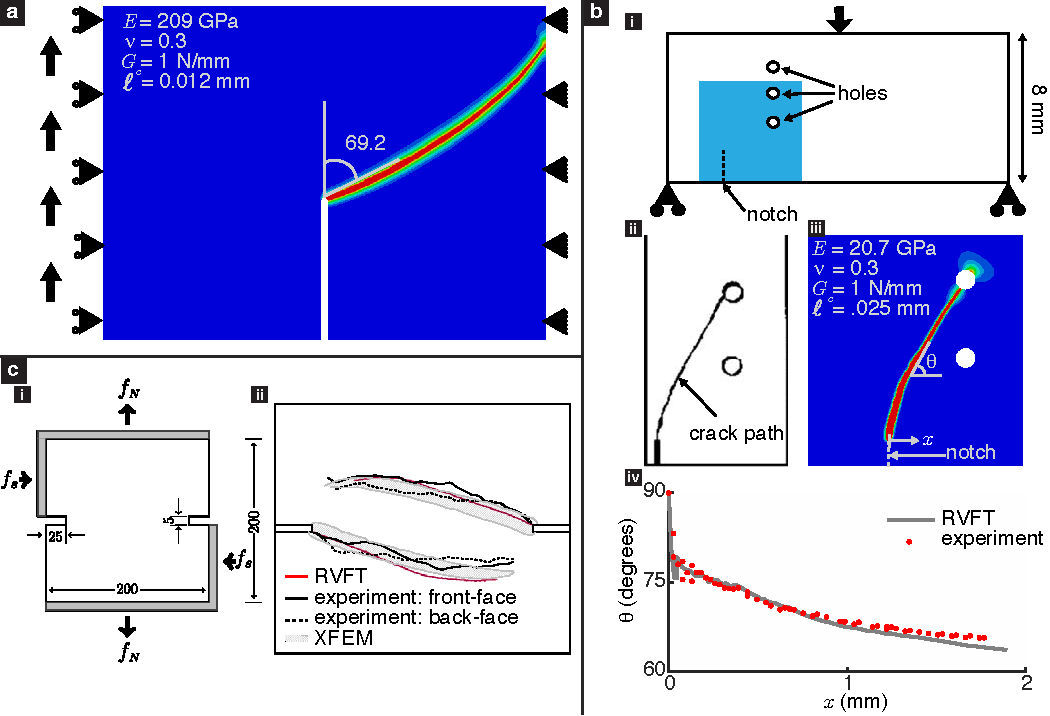
\includegraphics[width=\textwidth]{./Figure1_box_ver8.pdf}
	\caption{(a) Crack path under mode-II shear loading predicted by RVFT. The red region indicates the crack where the damage variable $d=1$. (b) In subfigure (i) the geometry and loading conditions for a bar with three holes drilled in it are shown. The experimentally observed crack path and crack path predicted by RVFT are shown in subfigures (ii) and (iii), respectively. The angle $\theta$ of the crack path for both the experimental results and RVFT prediction are shown in subfigure (iii). (c) Quantitative comparison of RVFT predictions and experimental results for mixed mode loading (adapted from \cite{mesgarnejad2015validation}). The loading conditions of the experiment conducted by \cite{nooru1992mixed} are shown in subfigure (c.i). The crack path from the experiments (shown as black dashed curves) is in good agreement with RVFT predictions (shown in red) obtained by \cite{mesgarnejad2015validation}. The XFEM results shown as grey curves are from \cite{bobinski2014constitutive}.}
	\label{Fig4}
\end{figure}


We appreciate the Reviewer's interest in comparing results from the RVFT to those obtained from tests performed on synthetic analogs of the spicules. We believe that further investigation of the cylindrical layered architecture through the use of synthetic analogs would give deeper insights into the toughening mechanisms acting within the spicules. Furthermore by varying the curvature of the layers one may be able to better understand the transition of toughening mechanisms from those operating in planar layered architectures to those operating in cylindrical layered architectures. However, we believe that this type of parametric study is outside the scope of the current work.

\item \label{r2c2} {\bf ``Furthermore, given the main gist of the discussion lies on the insights gained from the computational results, are there any limitations to point out on the validity of application of the VFM?''}

We appreciate the Reviewer's healthy skepticism of the RVFT as an investigative tool. In the supplementary information related to the RVFT (Section 4.1) we made sure to identify what we believe is the biggest issue underlying the RVFT---that the solution displacement field and crack(s) are postulated to be global minimizers of the system's total potential energy rather than local minimizers. However, like the Reviewer has suggested, there are other limitations to the RVFT as well. For example, the RVFT as formulated in Section S4 can only be used when the material(s) in the model are both linear elastic and brittle (i.e., they have a small fracture process zone). These limitations are not problematic for the current work since (i) results from a previous study \cite{monn2017enhanced} show that the spicules behave in a linear elastic fashion, and (ii) fractography performed in the current work (see Section 2.2 and Figure 6) does not show a large process zone or region of inelastic behavior.

However, in our opinion, the biggest limitation of RVFT is that it is computationally expensive. As a result of this limitation it is quite difficult to simulate the behavior of complex architectures or architectures with many repeating units (e.g., materials like nacre that contain hundreds of layers each consisting of many tablets). This is the primary reason that we only modeled two layers in the representative planar and cylindrical layered architectures described in Section 3 of the paper.

In response to this comment we have made one change, which is listed as \ref{Mc1} in the \textit{LoC}.
%
Through change \ref{Mc1} we have added a new paragraph to Section S4.1 in which we describe this major limitation of RVFT (computational expense) and how it limits our ability to model the exact architectures of different stiff biological materials.

\item \label{r2c3} {\bf ``The term `specific fracture initiation toughness', an important concept the authors build upon in this work, initially appears in the fourth line of the text, but its formal definition comes to light only at pag 4. I suggest providing an informal definition of this term right when it appears for the first time. It doesn't need to be technical (at pag 4 there is already one), yet a few words to clarify the reader of this journal of broad audience what the authors refer to would certainly be an asset.''}

We agree with the Reviewer that the concept of fracture toughness should be defined earlier in the manuscript. In response to this comment we have made one change, which is listed as \ref{mc1} in the \textit{LoC}.
%
Through change \ref{mc1} we have added a new sentence in the first paragraph of the introduction that provides a basic definition of fracture toughness.

\item \label{r2c4} {\bf ``Figure 3. i) Fig 3A. although quite clear, I would suggest adding the standard dash-dot line on the specimen geometry in A and B to indicate exactly where the circular cross-sections below are taken. ii) Fig 3C. References missing. I recommend including references in the caption for the data therein plotted. iii) Fig 3A seems uncalled in the text. The first instance I see is only for Fig 3B and 3C at line 58.''}

In response to this comment we have made one change, which is listed as \ref{mc2} in the \textit{LoC}.
%
Through change \ref{mc2} we have added the standard dash-dot line in subfigures 3A and 3B to indicate the location of the cross-sections. We have also added a reference to Figure 3A in the fourth paragraph of the introduction. Finally, we have identified the references from which the data in Figure 3C were obtained in the caption.

\item \label{r2c5} {\bf ``Figure 8. It seems the y axis is on log scale. If this is the case, I suggest indicating it on the axis and/or in the caption. In addition, also Fig 8A is not referenced in the text, only Fig 8b is at line 240.''}

In response to this comment we have made one change, which is listed as \ref{mc3} in the \textit{LoC}.
%
Through change \ref{mc3} we have modified the caption of Figure 8 to point out that the vertical axis has a logarithmic scale. We thank the Reviewer for this suggestion and think that pointing out that the vertical axis has a log scale reinforces the overall message of our work. We have also added a reference to Figure 8A in the test (in the fourth paragraph of the introduction). Finally, we have identified the references from which the data in Figure 3 C were obtained.

\item \label{r2c6} {\bf ``Figure 9. There seems to be an inconsistency with the choice of the view in Fig 9A and Fig 9B, the former displaying an axonometric view, whereas the latter is unclear (is it a front view?) because the cross-section on its right is a circle. How can this be? It should be an ellipse in an axonometric view, or I am missing something here. Another point on Fig 9F. Why at the notch location (bottom) a brown shaded zone appears? What is the physical meaning? Should the notch appear as open, as it is visible in the corresponding fig. 9D?''}

In response to this comment we have made one change, which is listed as \ref{mc4} in the \textit{LoC}.
%
Through change \ref{mc4} we have modified Figure 9B so that it is an axonometric view and have removed the brown shaded zone at the notch in Figure 9F. The Reviewer is correct that the notch should appear as open like in Figure 9D. The brown zone in the original Figure 9F was an error that resulted from unintentionally extrapolating the solution outside of the domain of our model. We thank the Reviewer for pointing out these mistakes.


\item \label{r2c7} {\bf ``Statistics. This is a general comment that should be applied to relevant plots, table as well as text populated with data from this work or from the references. Statistical values are recommended for inclusion, where possible of course (if no data from the literature are available then the authors should nevertheless state this). The authors do a good job in providing mean values and standard deviations for the relevant mechanical property, e.g. line 173, but these values should be included also for the specimen geometry, so as to capture any discrepancy that might exist. For example, the start of the results section reports 25 Ea. and 12 Ta. Spicules were flexurally tested. But it seems no information (or I couldn't see) is given on the distribution of the geometric parameters that define these specimens. I would suggest including such information. I see much later in the text (pag 10) relevant values on the radius of curvature of the notch are given. Yet my comment here applies to the other main descriptors of the specimen geometry (cross-section radius, spicule length, layers thickness etc..). I would suggest including values of the specimen geometry up front in the results section, and use these raw values to build a short paragraph on the `specimen geometry characterization' showing any variations between data.''}

In response to this comment we have made three changes, which are listed as \ref{Mc2}--\ref{Mc4} in the \textit{LoC}.
%
Through change \ref{Mc2} we have included a new table (Table 1 in the revised version) that provides statistical data for our measurements of diameter, span, and notch length for both the \textit{E. aspergillum} and \textit{T. aurantia} spicule specimens.
%
Through change \ref{Mc3} we have added the standard error of the notch root radius measurements to paragraph 4 of Section 2.3. This completes the inclusion of statistical data for specimen geometry.
%
Through change \ref{Mc4} we have modified Table 2 in the revised version (Table 1 in the original version). This table contains the crack growth resistance data (both $R(0)$ and $\left< R\right>$) used to compute the toughness metrics in Figure 8 for nacre, bone, antler, and conch shell. We have added statistical data such as mean, standard deviation, and sample number, when available. We have also clarified in the table notes when the number of specimens was not provided by a given reference or when the values in the table were estimated from graphs. We appreciate the Reviewer pointing out this deficiency in our work.

\item \label{r2c8} {\bf ``A similar recommendation applies to the plot in S1 where the effect of moisture on the mechanical properties is given for 33 dry Ea and 11 wet Ea spicules. I suggest including in the caption the statistical output of the experiments to corroborate the claim that no difference in Young's modulus and strain failure emerges from the testing results. On this point, I also note here that the scatter of the green and the light blue bars shows some differences. Can the authors expand on the reasons please?''}

In response to this comment we have made one change, which is listed as \ref{mc5} in the \textit{LoC}.
%
Through change \ref{mc5} we have added the mean and standard error for the Young's modulus and bending failure strain of the wet and dry \textit{E. aspergillum} spicules to the caption of Figure S1. The statistical treatment of this data is handled in more detail in Section S2, where we use both bias-corrected accelerated confidence intervals and two-sided $t$-tests to corroborate our claim that there is no significant difference in effective Young's modulus or bending failure strain between the dry and wet spicules.

The difference in the scatter between the dry and wet spicules is most likely a consequence of the difference in sample number. That is, we only tested 11 spicules that were soaked in artificial seawater compared to the 33 dry spicules that were tested in \cite{monn2017enhanced}. The effect of hydration on the mechanical behavior of the \textit{E. aspergillum} spicules is certainly an important research topic, but a more in-depth treatment is beyond the scope of this work.

\item \label{r2c9} {\bf ``Line 76. The sentence `orthonormal set of Cartesian basis vectors $\{$e\string^1, e\string^2, e\string^3$\}$, shown in Figure 4 (A), (B), and (D), and their corresponding Cartesian coordinates $\{$x1, x2, x3$\}$'. Since fig 4 reports only the basis vectors without any display of the system $\{$x1, x2, x3$\}$, I would suggest to slightly amend the sentence as `orthonormal set of Cartesian basis vectors $\{$e\string^1, e\string^2, e\string^3$\}$ (Figure 4 (A), (B), and (D)), which correspond to the Cartesian coordinates $\{$x1, x2, x3$\}$'.''}

In response to this comment we have made one change, which is listed as \ref{mc6} in the \textit{LoC}.
%
Through change \ref{mc6} we have modified the sentence so that it now reads ``The spicule specimen's undeformed configuration can be described using the orthonormal set of Cartesian basis vectors $\{\ex,\ey,\ez\}$ (Figure 4 (A), (B), and (D)), which correspond to the Cartesian coordinates $\{x_1,x_2,x_3\}$.''

\item \label{r2c10} {\bf ``Minor typos
In the main text: Line 276 layers, like that which appear >> like those? In the supplementary information: Line 14. That that >> avoid duplicate, Line 39. compare >> compared, Line 340. have been soaked >> were soaked, Reference 2 in the supplementary information lacks some data, such as the year.''}

In response to this comment we have made one change, which is listed as \ref{mc7} in the \textit{LoC}.
%
Through change \ref{mc7} we have corrected the typos identified by the Reviewer. We thank the Reviewer for identifying these small mistakes and allowing us to improve the quality of the manuscript.

\end{enumerate}

\clearpage
%%%%%%%%%%%%%%%%%%%%%%%%%%%%%%%%%%%%%%%%%%%%%%%%%%%%%%
\section*{Response to Reviewer \#3's comments}
\label{rev3}

% STOPPED HERE 8/12/19
\begin{enumerate}[label=\textit{3.\arabic*},wide, labelwidth=!, labelindent=0pt]
\item \label{r3c1} {\bf ``Now the authors gave an fairly extensive review on the studies reported until today by focusing on the toughness issues. However what I criticize is that the selection of the papers they cite is very ambiguous. The groups e.g. of Mayer, Fratzl, Weiner gave detailed report on this issue. Some pertinent report of these groups and also from others highlighted the importance of the proteins within the silica spicules and from the inter-layers.''}

Since this work focuses on the toughness properties of the \EA spicule, we focused our review on previous works that do the same. Many of these works have been published by Professor Mayer's group and are listed as references 5, 6, and 16 in the revised version of the manuscript. We do not agree that these references are ambiguous because, to our knowledge, they represent the main contributions to the study of the \EA spicules from the perspective of toughness enhancement via experimental measurements. The toughness properties of spicules with layered architecture produced by other species of the class Hexactinellida have been explored in references 19--22 and 54 in the revised version of the manuscript.

We agree with the Reviewer that Professor Fratzl's group and his collaborators (such as Professor Kolednik) have also made significant contributions to this subject. Their works primarily focus on modeling the effects of an elastically heterogeneous, layered architecture on initiation toughness. They propose a crack tip shielding effect that is caused by the interaction between a crack and an elastic heterogeneity. Through change \ref{Mc04} listed in the \emph{Loc} we have added an additional discussion of these works to Section 2.3 in the revised version of the manuscript. In this discussion, we describe the main premise of these models for toughness enhancement and point out how the analysis that we present in Section 2.5 constitutes a novel contribution by considering the cylindrical geometry of the \EA spicule's architecture. We have included references to the contributions of these groups, which are listed as references 8, 25, and 45--47 in the revised version of the manuscript.

To our knowledge Professor Weiner's group has not published any works on siliceous spicules (i.e. Demosponge or Hexactinellid spicules). Consequently, we have not included a review of their works in this manuscript. However, we do not deny the importance of the protein scaffold within the spicule's silica nor the composition of the interlayers. Our review of this topic focuses on the contributions of Dr. Weaver and Professor Aizenberg which are listed as references 17, 18, 43, and 54 in the revised version of the manuscript. These works describe the composition and nanoscale structure of the spicules' silica. We revisit the importance of the protein scaffold and composition of the silica itself in the final paragraph of Section 2.5. In this paragraph we point out that we chose the \TA spicules as a homogeneous control material based on the similarity of their composition and the composition of the \EA spicules. We admit that the best choice for this homogeneous control material would be the core of the \EA spicules themselves. However, we point out the difficulty of obtaining core samples large enough to test.

\item \label{r3c2} {\bf ``Also---importantly they mix spicules from demosponges with those from hexactinellids. This is not justified since the structure, composition of those spicules is different between these two taxa.''}

We agree that using spicules from the same taxonomic class would be the ideal choice. In fact, in Section 2.5 we state that ``The \EA spicules should instead be compared to a specimen composed of the same biogenic silica but which is monolithic. An ideal choice for this homogeneous control material would be a section of the solid silica core of the \EA spicules. However, so far we have not successfully obtained a large enough section of the \EA spicule core to perform fracture tests. Therefore, we chose the \TA spicules as what we believe to be the next best alternative.''

We used the \TA spicules specifically as a material for comparison since they have been shown to have a similar volume-averaged bonding structure to the \EA spicules \cite{weaver2010unifying}. Specifically, $^\text{29}$Si MAS NMR spectra of the \EA and \TA spicules indicate no distinguishable differences in the condensation of their silica. While this does not rule out differences in the proteinaceous scaffold, it does give a clear indication that the \TA spicules are a close approximation in terms of silica composition. We have also measured the Young's moduli of both the \EA and \TA spicules via three-point bending tests and found no significant difference between the two. This indicates that the elastic moduli of the silica from the \EA and \TA spicules are similar.

We agree with the Reviewer that differences in spiculogenesis between hexactinellids and demosponges will cause structural differences between the \EA and \TA spicules. We believe that this work constitutes a substantial improvement over past works focusing on toughness because it is the first to compare the \EA spicules to spicules from a related sponge instead of to synthetic glass. We hope that this work will motivate the importance of continuing to seek better control materials for comparison, such as sections of the \EA spicule core.

\item \label{r3c3} {\bf ``I the authors would stick to one taxon---then they surely will come to another conclusion. Then the issue, basically two issues, become more clear.''}

We do not know what two issues the reviewer is referring to. 

Regarding the conclusions of our work, we can assess the \EA spicule's toughness enhancement by analyzing the data we present for the \EA spicules alone. Specifically, by taking the ratio of $\left< R\right>$ to $R(0)$ for the \EA spicules we can quantify the rise in their $R$ curve during the propagation of a crack. This gives a rough sense of the effect of the \EA spicule's architecture on its toughness during crack propagation through what are considered ``extrinsic'' toughening mechanisms (see \cite{evans1990perspective}). For the \EA spicules, this ratio is approximately 22. We can compute this ratio for other biological materials using values found in Table 2. The values of $\left< R\right>/R(0)$ for nacre, bone, antler, and conch are 3.5, 56.3, 140.0 and 1040.0, respectively. Thus, even without comparing to the \TA spicules we can see that the increase in $R$ provided by the \EA spicule's architecture is significantly smaller than most of these other biological materials.

\item \label{r3c4} {\bf ``I do not see any new ideas on the toughness of the layered mineralic biomaterials.''}

Many previous studies have suggested that the \EA spicules' layers enhance toughness like the layers observed in other mineralized biological materials \cite{mayer2011new, mayer2005rigid, walter2007mechanisms, kolednik2011bioinspired}. This has been the dominant narrative in the field when discussing the functional implications of the \EA spicule's layers. The hypothesis that the \EA spicule's layers enhance toughness has led to the development of models that describe new toughness enhancement mechanisms in layered materials \cite{kolednik2014improvements, kolednik2011bioinspired, fratzl2007hindered}. 

This work provides experimental evidence of the contrary. Specifically, we show that the \EA spicule's layered architecture provides only modest enhancements to fracture toughness (both during initiation and propagation), especially compared to other biological materials like shell and bone. The stark contrast between the toughness enhancements observed in the \EA spicules and in these other materials demonstrates that the details of a material's layered architecture (e.g., flat vs cylindrical layers) can have extreme consequences on the toughening mechanisms that it enables and the resulting toughness enhancement it provides. Therefore, this work provides an entirely new perspective on the connection between the \EA spicule's layered architecture and its fracture toughness.

More importantly, this shows that not all layered architectures are created equal. This is critical for the bio-inspiration community because efforts to develop new high-toughness composite materials are often guided by the characterization of biological composites and subsequent identification of which architectures provide the best combinations of strength and toughness.

\item \label{r3c5} {\bf ``The authors gave a very attractive title for their manuscript---but they failed to give the readers an answer to: ``\ldots or a Siren Song.'' Just to mention that more conclusive results have to be worked out in the future is not sufficient.''}
\end{enumerate}

The title of the manuscript is meant to reflect the contrast between our findings and the widespread belief that biological materials with layered architectures have extraordinary fracture toughness. While we do state that ``the contrast between our findings and previous speculations that the \EA spicule's layers enhance their toughness shows that the understanding of the relationship between layered architectures and toughness enhancement is not yet complete'', we provide much more concrete conclusions as well. We enumerate some of the most important conclusions below.
%
\begin{enumerate}
    \item The \EA spicule's cylindrically layered architecture provides up to 10 fold increase in fracture initiation toughness. While this is certainly significant, it pales in comparison to the 250 fold increase observed in nacre (see Figure 8 (a)).
    \item Perhaps more importantly, the increase in average crack growth resistance provided by the \EA spicule's architecture is up to 3 orders of magnitude smaller than the enhancements provided by architectures with flat layers (see Figure 8 (b)).
    \item Using a regularized variational fracture method, we found that interfacial fracture is the dominant toughening mechanisms in the cylindrical layered architecture, but that its effect is small compared to the arrest and re-nucleation mechanism that occurs in a planar layered architecture.
\end{enumerate}
%
We do not believe that the answer to the question posed in our title (i.e., are architectures in stiff biological materials a template for toughness or a siren song?) has a single, definitive answer. In conch shell, the crossed lamellar architecture clearly provides extraordinary enhancements to average crack growth resistance. In nacre, the brick and mortar architecture does the same for fracture initiation toughness. In the \EA spicules, the cylindrically layered architecture only provides modest enhancements to both. While at first glance, all of these materials have similar architectures, however, the seemingly small architectural differences lead to quite different fracture toughness properties. Sometimes these properties are extraordinary, sometimes they are not. That subtlety is the main point of this work.

\clearpage
%%%%%%%%%%%%%%%%%%%%%%%%%%%%%%%%%%%%%%%%%%%%%%%%%%%%%%
\bibliographystyle{naturemag_noURL}
\bibliography{revbib}
\end{document}